\documentclass[a4paper, 12pt]{article}

\usepackage[portuges]{babel}
\usepackage[utf8]{inputenc}
\usepackage{amsmath}
\usepackage{indentfirst}
\usepackage{graphicx}
\usepackage[colorinlistoftodos]{todonotes}
\usepackage{float}

\usepackage[pdftex]{hyperref}




\begin{document}
%\maketitle

\begin{titlepage}
	\begin{center}
		\huge{Universidade Federal de Ouro Preto}

\vspace{10pt}
\begin{figure}[H]
\centering

\includegraphics[width=4cm]{img/logo.jpg}
\end{figure}
        
        \vspace{85pt}
        
		\textbf{\LARGE{Engenharia de Software II}}\\
		\large{Sistema de \textit{Empréstimo de Jogos}\\ Grupo: \textit{cafeína++;}}
		\vspace{160pt}
		
	\end{center}
	
	\begin{flushleft}
		\begin{tabbing}
			Alunos:\qquad\qquad\= Caio Soares Costa \\
			\>Cibele Oliveira Ferreira \\
            \>Eduardo Matosinhos Florinda \\
            \>Gabriel Caetano Araújo \\
			Professor:\> Johnatan Oliveira \\
			Horário:\> Seg e Qua - 08:20 - 10:00\\
		
	\end{tabbing}
		  
	\end{flushleft}
	
	\begin{center}
		%\vspace{\fill}
		Ouro Preto, \today
	\end{center}
\end{titlepage}
%%%%%%%%%%%%%%%%%%%%%%%%%%%%%%%%%%%%%%%%%%%%%%%%%%%%%%%%%%%
\newpage
\tableofcontents
\thispagestyle{empty}

\newpage
\pagenumbering{arabic}

%%%%%%%%%%%%%%%%%%%%%%%%%%%%%%%%%%%%%%%%%%%%%%%%%%%%%%%%%
%%%%%%%%%%%%%%%%%%%%%%%%%%%%%%%%%%%%%%%%%%%%%%%%%%%%
\section{Histórico de Revisões}

\begin{table}[H]
\centering
\begin{tabular}{|l|l|l|l|}
\hline
\multicolumn{1}{|c|}{Data} & \multicolumn{1}{c|}{Versão} & \multicolumn{1}{c|}{Descrição}                 & Autor       \\ \hline
10/03/2021                 & 0.0                         & Justificativa do processo de software          & Eduardo     \\ \hline
10/03/2021                 & 0.0                         & Levantamento de requisitos                     & Caio, Cibele e Gabriel            \\ \hline 
20/03/2021                 & 0.0                         & Especificação de requisitos                     & Caio, Cibele e Gabriel            \\ \hline
31/03/2021                  & 0.0                        & Requisitos a serem testados                 & Eduardo                            \\     \hline 
\end{tabular}
\caption{Revisões do Documento}
\label{tab:my-table}
\end{table}

\section{Processo e Software}
% Apresente aqui uma breve explicação do modelo de processo de software escolhido. Lembre-se, vocês precisam citar claramente o modelo de processo de software escolhido, por exemplo, \textbf{SCRUM}.

A equipe ‘‘cafeína++;’’, desenvolvedora do software ‘‘Game Stonks’’, adotou o processo de desenvolvimento ágil Scrum. Esta escolha levou em consideração o fato deste modelo permitir a criação de um software útil rapidamente. Desta forma, desenvolvemos o sistema por uma série de incrementos, em que os usuários finais ou o representante do cliente participam da especificação e validação de cada incremento, garantindo o alcance da maior satisfação do cliente. Em termos teóricos ele se baseia em três pilares, transparência, inspeção e adaptação. Ou seja, todos os papéis, eventos, artefatos, propósitos e valores, são para dar visibilidade ao trabalho em questão, permitir uma validação antes, durante e depois do processo e a qualquer momento realizar ajustes nas demandas a serem executadas.

\section{Cronograma}
% Vocês devem apresentar aqui o cronograma das atividades e seus respectivos responsáveis. 

\begin{table}[H]
\centering
\begin{tabular}{|l|l|l|}
\hline
\multicolumn{1}{|c|}{Nome} & \multicolumn{1}{c|}{Tarefa}                                                                                   & \multicolumn{1}{c|}{Prazo} \\ \hline
Eduardo                    & Definir tema do projeto                                                                                       & 01/03  \\ \hline
Gabriel                    & Criar repositório no GitHub                                                                                   & 01/03  \\ \hline
Eduardo                    & \begin{tabular}[c]{@{}l@{}}Escolha e justificativa do Processo de \\ Desenvolvimento de Software\end{tabular} & 13/03  \\ \hline
Caio, Cibele e Gabriel     & Levantamento dos requisitos do software                                                                       & 13/03  \\ \hline
\begin{tabular}[c]{@{}l@{}}Caio, Cibele e\\ Gabriel \end{tabular}     & Especificação de requisitos                               & 20/03  \\ \hline
Gabriel                    & Definição da tecnologia, arquitetura e classes                                                                & 20/03  \\ \hline
\begin{tabular}[c]{@{}l@{}}Caio, Cibele, Eduardo e\\ Gabriel \end{tabular} & Definir backlog                                               & 24/03  \\ \hline

\end{tabular}
\caption{Cronograma}
\label{tab:my-table}
\end{table}

\section{Levantamento de Requisitos}
% Independente da metodologia de desenvolvimento utilizada, o levantamento de requisitos é o ponto de partida de qualquer projeto de software, pois é a partir dos resultados obtidos durante esta etapa que será possível definir como as próximas etapas do desenvolvimento serão executadas.

% Apresente a técnica que a sua equipe irá utilizar, explique porquê de tal técnica e quais os resultados obtidos.
\subsection{Diagrama de Caso de Uso}

\begin{figure}[H]
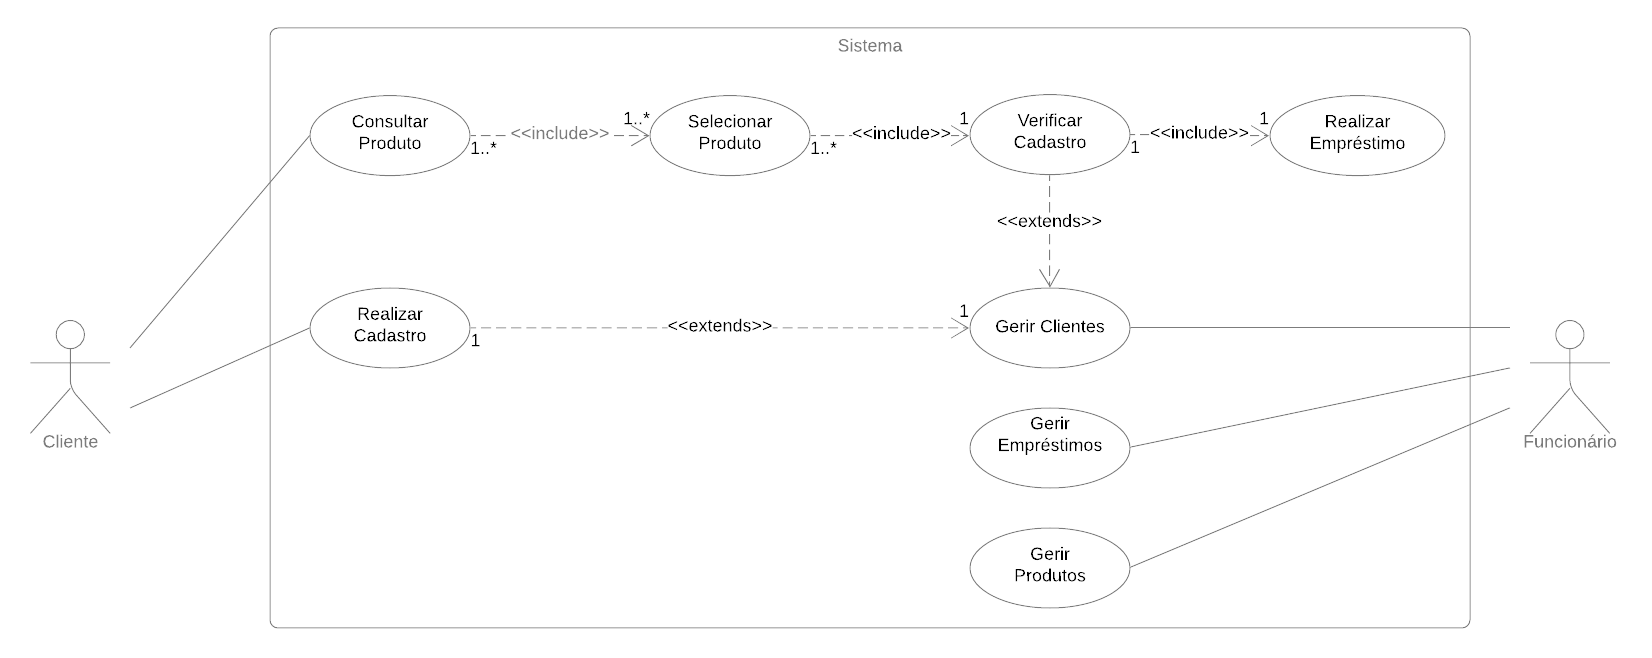
\includegraphics[width=\textwidth]{./img/casos-de-uso.png}
\centering
\caption{Diagrama de Casos de Uso}\label{img:casos-de-uso}
\end{figure}

\subsection{Descrição de Caso de Uso}

\begin{table}[H]
\centering
\begin{tabular}{|l|l|l|}
\hline
\multicolumn{1}{|c|}{Código} & \multicolumn{1}{c|}{Serviço} & \multicolumn{1}{c|}{Descrição} \\ \hline
RF01  & Realizar cadastro   & \begin{tabular}[c]{@{}l@{}}Permite o cliente se cadastrar no sistema. \end{tabular} \\ \hline
RF02  & Consultar produtos  & \begin{tabular}[c]{@{}l@{}}Permite o cliente consultar um jogo no \\ sistema. \end{tabular} \\ \hline
RF03  & Selecionar produto  & \begin{tabular}[c]{@{}l@{}}Permite o cliente selecionar um jogo para \\ empréstimo. \end{tabular} \\ \hline
RF04  & Verificar cadastro  & \begin{tabular}[c]{@{}l@{}}Possibilita a verificação do cadastro do cliente \\ no sistema. \end{tabular}  \\ \hline
RF05  & Realizar empréstimo & \begin{tabular}[c]{@{}l@{}}Efetiva o empréstimo do produto para o cliente \\ que o selecionou.\end{tabular}  \\ \hline
RF06  & Gerir clientes      & \begin{tabular}[c]{@{}l@{}}Gerencia os clientes que estão cadastrados no \\ software. \end{tabular}  \\ \hline
RF07  & Gerir empréstimos   & \begin{tabular}[c]{@{}l@{}}Gerencia os empréstimos realizados.\end{tabular}  \\ \hline
RF08  & Gerir produtos      & \begin{tabular}[c]{@{}l@{}}Gerencia os produtos (jogos) do software. \end{tabular}  \\ \hline

\end{tabular}
\caption{Descrição de Casos de Uso}
\label{tab:descricao-casos-de-uso}
\end{table}

% \textit{Para o levantamento de requisitos, o analista dispõe de algumas técnicas que são utilizadas de acordo com o perfil do cliente. Existem diversas técnicas, cada uma adequada para um cenário específico, e dentre as comumente utilizadas podemos citar as seguintes técnicas:}

% \begin{enumerate}
% \item Descoberta de Requisitos  (Pontos de vista)
% \item Entrevistas
% \item Cenários
% \item Casos de Uso
% \item Etnografia 
% \end{enumerate}

\section{Especificação de Requisitos}
\subsection{Requisitos Funcionais}
\textbf{RF01--} \textbf{Realizar cadastro:} Este serviço realiza todas as tarefas relacionadas à autenticação.
\begin{itemize}
    \item \textbf{Criar login:} Campo de texto para login.
    \item \textbf{Criar senha:} Campo de texto para senha.
    \item \textbf{Recuperar senha:} Permite recuperar a senha.
    \item \textbf{Alterar senha:} Permite alterar a senha.
    \item \textbf{Autenticar login e senha:} Valida o login e senha.
    \item \textbf{Sair do sistema:} Realiza o logout.
\end{itemize}

\textbf{RF02--} \textbf{Consultar Produto:} Este serviço possibilita que o usuário consulte se o jogo que ele irá pegar emprestado está disponível.
\begin{itemize}
    \item \textbf{Filtrar Jogos:} Possibilita que o usuário filtre os jogos de acordo com tema, nome e empresa de desenvolvedora.
    \item \textbf{Consultar Disponibilidade:} Possibilita que o usuário veja se um jogo estará disponível para empréstimo.
\end{itemize}

\textbf{RF03--} \textbf{Selecionar Produto:} Este serviço permite ao usuário adicionar um jogo ao carrinho para o empréstimo.

\begin{itemize}
    \item \textbf{Adicionar Jogo:} Permite adicionar jogos ao carrinho.
    \item \textbf{Remover Jogos:} Permite remover jogos do carrinho.
    \item \textbf{Atualizar valor de jogos no carrinho:} Atualiza o valor total dos jogos para empréstimo.
\end{itemize}

\textbf{RF04--} \textbf{Verificar cadastro:} Este serviço faz a verificação do cadastro do usuário e validação das informações
\begin{itemize}
    \item \textbf{Autenticação de login:} Verifica se o usuário está cadastrado no sistema antes de prosseguir com o empréstimo.
    \item \textbf{Autenticação de informações:} Verifica se as informações inseridas pelo usuário estão corretas.
    \item \textbf{Verificar pendências:} Verifica se o usuário possui algum débito registrado no sistema.
\end{itemize}

\textbf{RF05--} \textbf{Realizar Empréstimos:} Este serviço possibilita que o usuário efetue o empréstimo do jogo que deseja.
\begin{itemize}
    \item \textbf{Validar dados do cartão:} Valida os dados de cartão de crédito do usuário.
    \item \textbf{Efetuar pagamento:} Utiliza uma API para realizar o pagamento do empréstimo solicitado pelo usuário.
    \item \textbf{Liberar Empréstimo:} Disponibiliza para o usuário os jogos que ele escolheu por empréstimo.
\end{itemize}

\textbf{RF06--} \textbf{Gerir clientes:} Este serviço realiza todas as tarefas relacionadas ao cadastro de usuários do sistema.
\begin{itemize}
    \item \textbf{Cadastrar usuário:} Permite cadastrar um usuário no sistema.
    \item \textbf{Consultar usuário:} Permite visualizar todos os dados de um usuário registrado.
    \item \textbf{Buscar usuário:} Permite fazer uma busca de um usuário no sistema.
    \item \textbf{Alterar dados do usuário:} Permite atualizar todos os dados relacionados a um usuário.
    \item \textbf{Remover usuário:} Permite excluir o usuário do sistema.
\end{itemize}

\textbf{RF07--} \textbf{Gerir empréstimos:} Este serviço realiza todas as tarefas relacionadas à contabilidade de gastos e lucros do Game Stonks.
\begin{itemize}
    \item \textbf{Consultar empréstimos:} Permite ao administrador visualizar os empréstimos realizados.
    \item \textbf{Consultar lucro por jogo:} Permite ao administrador visualizar lucro por empréstimos de jogos.
    \item \textbf{Consultar resumo financeiro:} Permite ao administrador visualizar o resumo financeiro.
    \item \textbf{Exportar resumo financeiro:} Exporta relatório em formato CSV.
    \item \textbf{Registrar gastos com compra de jogos:} Permite que o administrador adicione os gastos com a compra de jogos.
    \item \textbf{Registrar lucro por jogo:} Permite que o administrador adicione os lucros por empréstimos de jogos.
\end{itemize}

\textbf{RF08--} \textbf{Gerir produtos:} Este serviço realiza todas as tarefas relacionadas ao gerenciamento dos jogos.
\begin{itemize}
    \item \textbf{Registrar jogos:} Permite que o administrador adicione as informações pertinentes aos jogos.
    \item \textbf{Consultar jogos:} Permite ao administrador visualizar os jogos cadastrados no sistema.
    \item \textbf{Editar jogos:} Permite ao administrador editar as informações dos jogos cadastrados no sistema.
    \item \textbf{Excluir jogos:} Permite ao administrador excluir jogos existentes no sistema.
\end{itemize}

\subsection{Requisitos Não Funcionais}
\textbf{RNF01.} A efetivação do empréstimo do jogo só deve ser liberada após o cliente estar
logado no sistema.
\textbf{Informações:} usuário e senha.
\textbf{Regras:} o cliente terá acesso para contratar, consultar e alterar. 

\textbf{RNF02} Compatibilidade com os sistemas operacionais Windows, Linux e MacOS.

\textbf{RNF03} Tempo limite para processamento de todas as solicitações de empréstimos de jogos.

\textbf{RNF04} Um visitante poderá visualizar os jogos que site tem disponível.
 
\textbf{RNF05} Informações pessoais dos usuários não podem ser vistas pelos operadores do sistema.


\section{Plano de VVT}

\subsection{Requisitos a serem testados}

\textbf{Teste de desempenho:} O objetivo deste teste consiste em validar se os requisitos de desempenho foram alcançados, como tempos de respostas e outros requisitos sensíveis ao tempo. Para isso deve-se:
\begin{itemize}
    \item Verificar tempo de resposta para login.
    \item Verificar a eficácia da aplicação do software diante de um aumento de acessos simultâneos.
    \item Verificar o tempo de resposta para atualizar o relatório financeiro diante das transações realizadas pelos usuários.
\end{itemize}

\textbf{Teste de segurança:} O objetivo deste teste consiste em verificar a proteção dos dados dos usuários do software, bem como revelar falhas e garantir a qualidade do software. Para isso deve-se:
\begin{itemize}
    \item Verificar possíveis falhas relacionadas a quebra de autenticação.
    \item Verificar se há proteção dos dados pessoais de todos os usuários.
    \item Verificar se há redirecionamento para sites maliciosos.
\end{itemize}

\textbf{Teste de interface de usuário:} O objetivo deste teste consiste em verificar se os componentes da interface estão respondendo às ações do usuário de maneira correta. Para isso deve-se:
\begin{itemize}
    \item Verificar funcionamento de botões.
    \item Tratar eventos de timeouts.
    \item Verificar se a navegação pelo aplicativo reflete os requisitos de negócios.
    \item Verificar se objetos da interface estão em conformidade com os padrões.
\end{itemize}

\subsection{Estratégias e ferramentas de teste}
\paragraph{Ferramenta Utilizada:} Jest é um framework de teste unitário de código aberto em JavaScript, sendo uma das ferramentas de teste unitário mais difundidas dentro da comunidade.
\subsubsection{Tipos de teste}
\paragraph{Teste Unitário:} O objetivo desse teste é verificar a adequadamente o processamento, recuperação dos dados e a funcionamento das estruturas implementadas. Esse tipo de teste baseia-se em técnicas de caixa branca, ou seja, usa a perspectiva interna do sistema, código fonte, para modelar os casos de teste.
\subparagraph{Técnicas Utilizadas:}
\begin{itemize}
    \item Executar para cada classe do sistema a instanciação de objetos, acesso aos métodos e atributos.
    \item Executar todos os métodos de cada classe do sistema verificando a validade dos resultados.
\end{itemize}
\subparagraph{Critérios de Conclusão:}
\begin{itemize}
    \item Todos os testes planejados foram executados.
    \item Todos os defeitos identificados foram tratados.
\end{itemize}

\subsection{Execução do Plano de Teste}
\subsubsection{Registrar Jogo}
\noindent
\textbf{Feature:} Testar a funcionalidade de registrar jogos. \\
\textbf{Cenário:} O administrador deseja realizar o cadastro de um jogo na sistema. \\
\textbf{Given:} O administrador informa os dados pertinentes aos jogos. \\
\textbf{When:} O administrador realiza o cadastro dos jogos no sistema. \\
\textbf{Then:} Os jogos são cadastrados no sistema.\\ 

\subsubsection{Registrar Cliente}
\noindent
\textbf{Feature:} Testar a funcionalidade de registrar clientes. \\
\textbf{Cenário:} O usuário deseja realizar um empréstimo no sistema e para isso precisa se registrar para prosseguir. \\
\textbf{Given:} O usuário informa seus dados pessoais para o cadrastro. \\
\textbf{When:} O usuário tenta realizar um empréstimo no sistema. \\
\textbf{Then:} O usuário preenche os campos com as informações solicitadas. \\

\subsubsection{Adicionar ao Carrinho}
\noindent
\textbf{Feature:} Testar a funcionalidade que cria o carrinho de empréstimo do usuário. \\
\textbf{Cenário:} O usuário irá selecionar os jogos que ele deseja pegar emprestado. \\
\textbf{Given:} O usuário deseja alugar alguns jogos. \\
\textbf{When:} O usuário tenta realizar um empréstimo no sistema. \\
\textbf{Then:} O usuário finaliza a seleção de jogos e fecha o carrinho. \\

\subsubsection{Efetuar Pagamento} 
\noindent
\textbf{Feature:} Testar a funcionalidade de efetuar os pagamentos dos serviços prestados pelo sistema. \\
\textbf{Cenário:} O usuário deseja efetuar o pagamento referente ao empréstimo de um jogo. \\
\textbf{Given:} O cliente adiciona um jogo ao carrinho. \\
\textbf{And:} O cliente possui saldo suficiente. \\
\textbf{When:} O cliente conclui a compra. \\
\textbf{Then:} O valor referente ao empréstimo é descontado no saldo do cliente. \\
\textbf{And:} A compra e o pagamento são efetuados com sucesso. \\

\section{Medição e Qualidade de Software}

O \textit{escomplex}\footnote{https://github.com/escomplex/escomplex} foi utilizado como ferramenta para ajudar na medição da qualidade do software. Essa ferramenta gera um relatório que tem um índice de complexidade do código escrito. Apesar disso, não se deve levar os resultados como valores absolutos para avaliar a complexidade do código desenvolvido. Algumas das métricas utilizadas por essa dependência são:

\begin{itemize}
    \item Linhas de código: físicas (o número de linhas em um módulo ou função) e lógicas (uma contagem das instruções imperativas).
    
    \item Número de parâmetros: Analisados estaticamente a partir da assinatura da função, portanto, nenhuma contabilização é feita para funções que dependem dos argumentos do objeto (quanto menor, melhor). 

    \item Complexidade ciclomática: É definida uma contagem do número de ciclos no gráfico de controle de fluxo do programa.
    
    \item Densidade de complexidade ciclomática: proposta como uma modificação da complexidade ciclomática, essa métrica simplesmente a reexpressa como uma porcentagem das linhas lógicas de código. (quanto menor, melhor).
    
    \item Medidas Halstead: Essas métricas são calculadas a partir do número de operadores e operandos em cada função (quanto menor, melhor).
    
    \item Índice de manutenção: É uma escala logarítmica de infinito negativo a 171, calculada a partir das linhas lógicas de código, a complexidade do ciclomatix e o esforço Halsteal (quanto mais alto, melhor).
    
    \item Densidade de primeira ordem: A porcentagem de todas as dependências internas possíveis que são realmente utilizados no projeto (quanto menor, melhor).
    
    \item Custo de mudança: A porcentagem de módulos afetados, em média, quando um módulo do projeto é alterado (quanto menor, melhor).
    
    \item Tamanho do núcleo: A porcentagem de módulos que são amplamente dependentes e dependem de outros módulos (quanto menor, melhor).
\end{itemize}

O \textit{JSHint}\footnote{https://jshint.com/docs/} é uma ferramenta de análise de código estática usada no desenvolvimento de software para verificar se o código-fonte JavaScript está em conformidade com as regras de codificação.

\newpage
\section{Referências}

[1] Sommerville, Ian -- Software Engineering, 8th Edition;

\end{document}